\documentclass{article}
\usepackage[utf8]{inputenc}
\usepackage[]{graphicx}
\usepackage[margin=1in]{geometry}
\usepackage{float}

\title{Circuits Lab 4}
\author{Theo Thompson and Dan Kearney}
\date{3.3.13}

\begin{document}

\maketitle

\section*{Experiment 1}

Our first experiment compared transistors on the same MAT14 transistor array. For each npn transistor, we tied the collector to the +5V power rail and grounded the emitter. We swept the base voltage from .25V to .65V to characterize the transistor. One way of measuring how well matched transistors are is to measure $\beta$ and $I_{s}$. To do this, we calculated the collector current using KCL: \[I_{e}=I_{b}+I_{c}\]
We then calculated $\beta$:\[\beta=\frac{I_{b}}{I_{c}}\]
To calculate $I_{s}$, we used the following relationship: \[I_{c}=I_{s}e^{\frac{V_{be}}{U_{t}}}\]
Where $V_{be}$ is the base-emitter voltage that we sourced with the SMU. The results of our calculation are summarized in the table below.
\begin{center}
    \begin{tabular}{| l | l |} \hline
    $\beta$ & $I_{s}$ \\ \hline \hline
    $875.52$ & $2.01*10^{-13}$ \\ \hline
    $875.64$ & $2.07*10^{-13}$\\ \hline
    $877.97$ & $2.10*10^{-13}$ \\ \hline
    $875.66$ & $2.07*10^{-13}$ \\ \hline
    \end{tabular}
\end{center}

Beta is very consistent across the four transistors. We calculated the standard deviation of $\beta$ to be $1.18$, which is about $.1\%$. The standard deviation of $I_{s}$ is $3.78*10^{-15}$, which is about $3.6\%$. These deviation values suggest that the transistors in the MAT14 transistor array are very well matched. To further investigate $\beta$ across all 4 resistors, we plotted $\beta$ as a function of base voltage in figure ~\ref{fig:exp1c}. The plot shows that $\beta$ is well matched across all operation regions of the transistors.
\begin{figure}[H]
\begin{center}
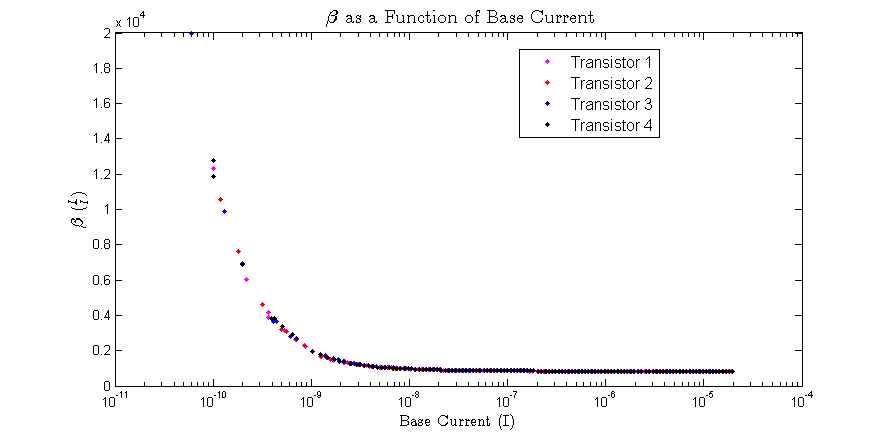
\includegraphics[scale=.8]{exp1c.png}
\caption{$\beta$ as a function of $V_{be}$ across all 4 devices.}
\label{fig:exp1c}
\end{center}
\end{figure}

Next, we wanted to investigate the similarity of currents between the devices. Figure ~\ref{fig:exp1a} shows the base and collector currents for all 4 transistors on the same plot. The currents are almost identical.

\begin{figure}[H]
\begin{center}
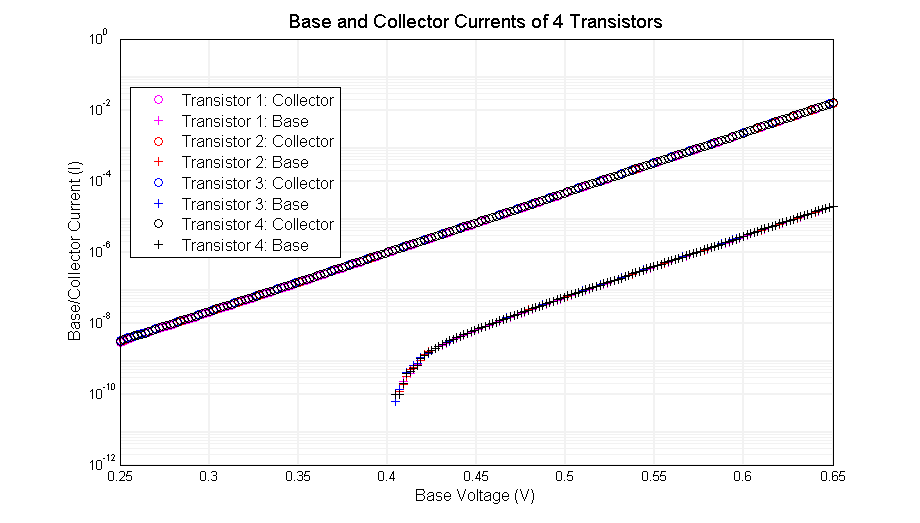
\includegraphics[scale=.6]{exp1a.png}
\caption{The base and collector currents of all 4 transistors in response to a base voltage sweep.}
\label{fig:exp1a}
\end{center}
\end{figure}

The similarity of the transistors' currents is better illustrated in figure ~\ref{fig:exp1b}. This plot shows the percentage difference of each transistor's collector current from the mean value. The collector currents are within a $2\%$ tolerance of the mean.

\begin{figure}[H]
\begin{center}
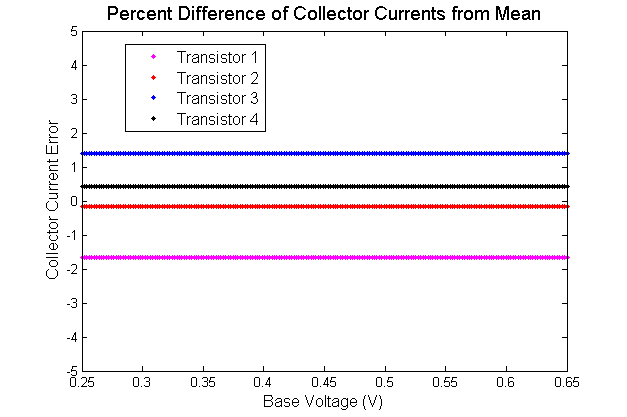
\includegraphics[scale=.6]{exp1d.png}
\caption{The percent error between each transistor's collector current and the mean value.}
\label{fig:exp1b}
\end{center}
\end{figure}

This experiment confirms that the transistors on the MAT14 are relatively very similar. This allows us to carry on with our experiments under the assumption that all 4 transistors are well matched.
\section*{Experiment 2}

In experiment 2, we analyzed the first translinear circuit, shown in Figure ~\ref{fig:tl1}.

\begin{figure}[H]
\begin{center}
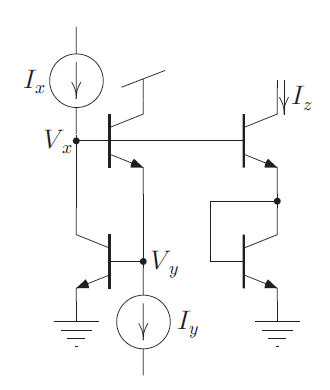
\includegraphics[scale=.5]{tl1.png}
\caption{Translinear circuit 1.}
\label{fig:tl1}
\end{center}
\end{figure}

\subsection*{Configuration 1: Sweeping $I_x$}

For our first configuration of the first circuit, we held the current $I_y$ constant using a current sink that we made using the circuit shown in Figure ~\ref{fig:sink}.  We sourced $I_x$ using the SMU and measured the current $I_z$ with the SMU as well.

\begin{figure}[H]
\begin{center}
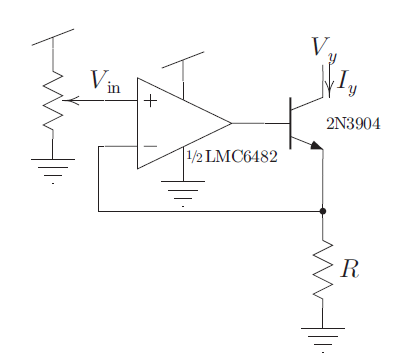
\includegraphics[scale=.5]{sink.png}
\caption{Our current sink.}
\label{fig:sink}
\end{center}
\end{figure}

\subsubsection*{The Current Sink}

We held that current sink constant by choosing our $V_{in}$ and our $R$ values such that we could produce a wide range of currents.  We knew from our prelab that the voltage at the base of the bottom-left transistor, $V_y$, will be approximately .6 V in forward-active mode.  Since the voltage will wiggle around .6 V, we needed the sink collector voltage, held at $V_{in}$ by the op-amp, to be underneath that by at least $V_{CEsat} \approx 200 mV$, so we chose a voltage that was well underneath it,  .1 V.

We generated .1 V at $V_{in}$ by using a voltage divider with resistor values 200 Ohms and 10k Ohms. Since our voltage source was 5 V, our resulting voltage at $V_{in}$ was .1 V.  

We used that voltage to generate a current through the current sink.  To generate 10 uA, by Ohm's law, we needed a resistor with resistance 10k $\Omega$; for 100 uA, 1k $\Omega$; for 1 mA, 100 $\Omega$.

\subsubsection*{Measurement}

We held $I_y$ constant and used the SMU to sweep $I_x$ over several orders of magnitude of current.   We did this for three values of $I_y$ that scaled three orders of magnitude.

From our prelab, we expect that this translinear circuit obeys the equation $I_x I_y = I_z ^2$.  As a result, when we hold $I_y$ constant, we expect $I_z = \sqrt{I_xI_y}$.  

Our experiment result, and our theoretical expectation, are shown in Figure~\ref{fig:exp2sweepx}.

\begin{figure}[H]
\begin{center}
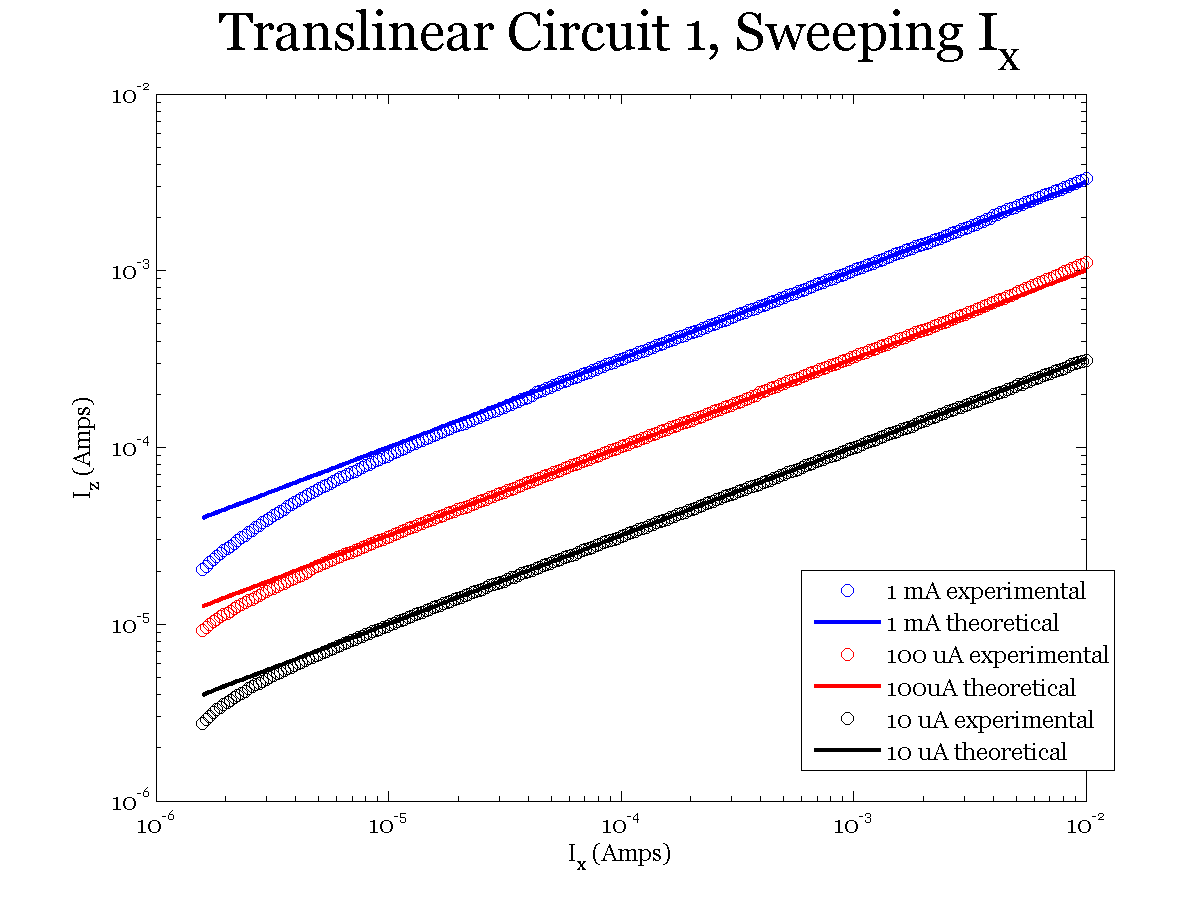
\includegraphics[scale=.75]{exp2_sweepx.png}
\caption{Translinear circuit 1, holding $I_y$ at the values shown in the legend.}
\label{fig:exp2sweepx}
\end{center}
\end{figure}

\subsubsection*{Error Analysis}

In general, this circuit behaves as we would expect from our analysis.  At small input currents, the output current is a little lower than expected, but we can expect that low currents are difficult for the SMU to write and read accurately.

\subsection*{Configuration 2}

Next, we took the same circuit from before and replaced the current sink with one channel of the SMU, such that we could sweep $I_y$, and held $I_x$ constant with a current source that we built.  Our current source is shown in Figure~\ref{fig:source}.

\begin{figure}[H]
\begin{center}
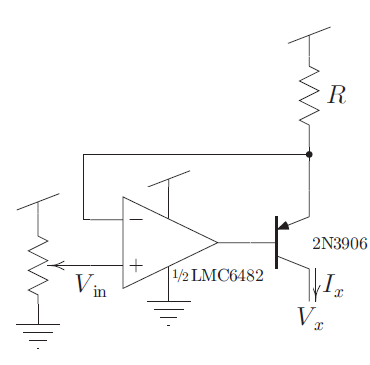
\includegraphics[scale=.5]{source.png}
\caption{Our current source.}
\label{fig:source}
\end{center}
\end{figure}

\subsection*{The Current Source}

We chose appropriate values of $V_{in}$ and R such that we could sweep our $I_y$ over several orders of magnitude, as in configuration 1.

For our voltage divider, we used a 2k $\Omega$ and a 3k $\Omega$ resistor to generate a voltage divider ratio of .4, and an output voltage of 3 Volts.

From the prelab, we know that our output current is $\frac{5 - V_{in}}{R}$.  To generate 1 uA, we used a 2 M$\Omega$ resistor; for 10 uA, 200 k$\Omega$; for 100 uA, 20 k$\Omega$.

\subsection*{Measurement}


Again, we expected, from the prelab, that $I_z = \sqrt{I_xI_y}$.  Our results are shown in Figure~\ref{fig:exp2sweepy}.

\begin{figure}[H]
\begin{center}
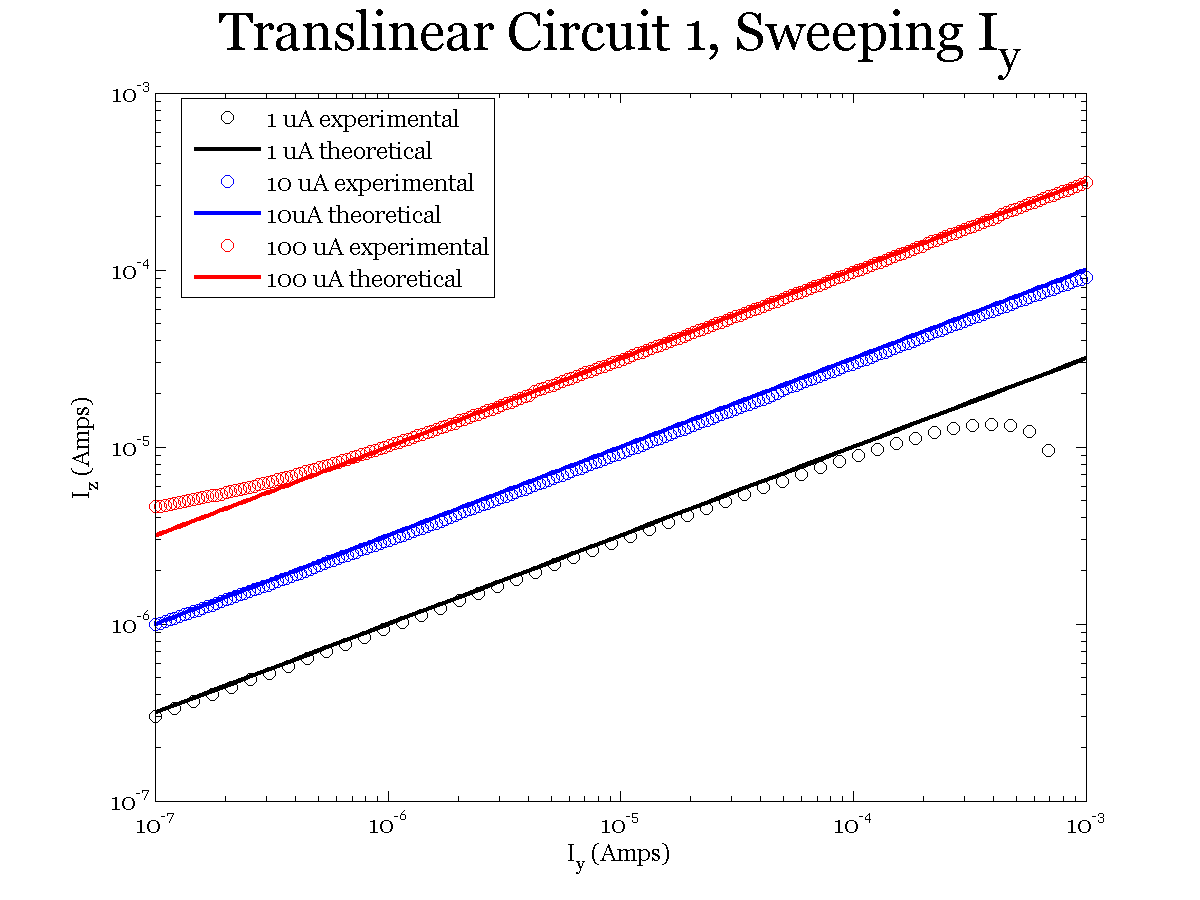
\includegraphics[scale=.75]{exp2_sweepy.png}
\caption{Translinear circuit 1, holding $I_x$ at the values shown in the legend.}
\label{fig:exp2sweepy}
\end{center}
\end{figure}

\subsection*{Error Analysis}

This circuit behaved well for low $I_x$ currents.  The expected and theoretical approaches are almost indistinguishable for $I_x = 10 \mu A$.  However, for high $I_x$, we found that the circuit broke down at high $I_y$ and started to decrease.  We believe that the dichotomy of very small measurement and very high output might have caused the SMU to fail.

\section*{Translinear Circuit 2}

We then repeated the experiments with a slightly different circuit, shown in Figure~\ref{fig:tl2}.


\begin{figure}[H]
\begin{center}
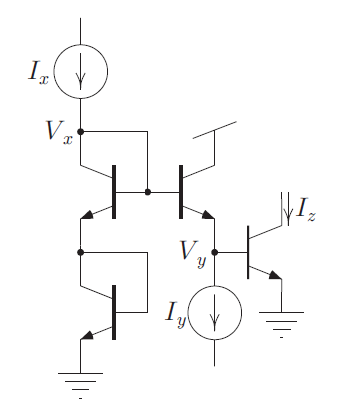
\includegraphics[scale=.5]{tl2.png}
\caption{Translinear circuit 2.}
\label{fig:tl2}
\end{center}
\end{figure}

As we did before, we used one channel of the SMU to sweep one of the currents in the circuit while holding the other current constant using current source or sink we built.

\subsection*{Configuration 1}

In the first configuration, we held $I_y$ constant with our hand-built current sink and swept $I_x$ with the SMU.  

\subsubsection*{The Current Sink}

This current sink was almost identical from the current sink we used in Translinear Circuit 1, but we desired a slightly different range of currents to make the transistors behave over three decades.  We used the same voltage divider to generate .1 V, but used a 200 k$\Omega$ resistor to generate 500 nA; for 5 uA, 20 k$\Omega$; for 50 uA, 2 k$\Omega$.

\subsubsection*{Measurement}

From the prelab, we expect this circuit to follow $I_x ^2 = I_z I_y$.  As a result, holding $I_y$ constant should yield $I_z = \frac{I_x^2}{I_y}$, which means that $I_z$ will increase linearly on a log-log scale as we sweep $I_x$.  Our results are in Figure~\ref{fig:tl2sweepx}.

\begin{figure}[H]
\begin{center}
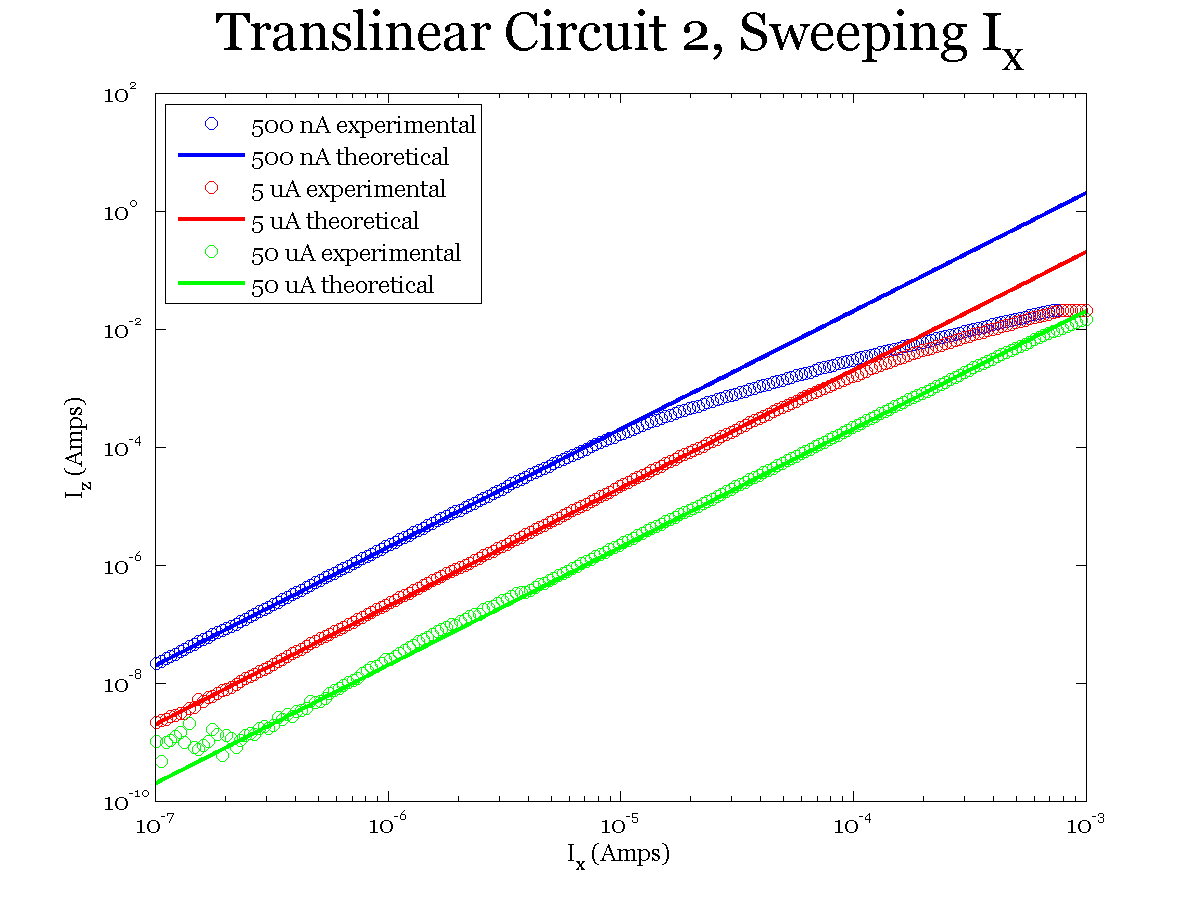
\includegraphics[scale=.75]{exp3_sweepx.png}
\caption{Translinear circuit 2, holding $I_y$ at the values shown in the legend.}
\label{fig:tl2sweepx}
\end{center}
\end{figure}

We swept over a high dynamic range (five orders of magnitude) and found that the data matched the theoretical expectation very well for the majority of the range of our input current values.  

\subsubsection*{Error Analysis}

We found that decreasing $I_y$ caused the current to increase more slowly as we increased $I_x$, which we can attribute to the difficulty in sourcing nanoamps of current while measuruing millamps of current.

\subsection*{Configuration 2}

We then switched our circuit around such that our current source was holding $I_x$ constant and the SMU swept $I_y$ over a high dynamic range.  Again, we expect $I_z = \frac{I_x^2}{I_y}$, which means that $I_z$ should decrease linearly on a log-log scale as we sweep $I_y$.  

\subsubsection*{The Current Source}

We used a similar current source to the one that we used in Translinear Circuit 1.  However, we swept over a slightly tighter dynamic range (about one and a half orders of magnitude).  To generate 22 uA, we used a 90 k$\Omega$ resistor; for 10 uA, 200 k$\Omega$; and for 100 uA, 20 k$\Omega$.

\subsubsection*{Measurement}

Our results can be seen in Figure~\ref{fig:tl2sweepy}.

\begin{figure}[H]
\begin{center}
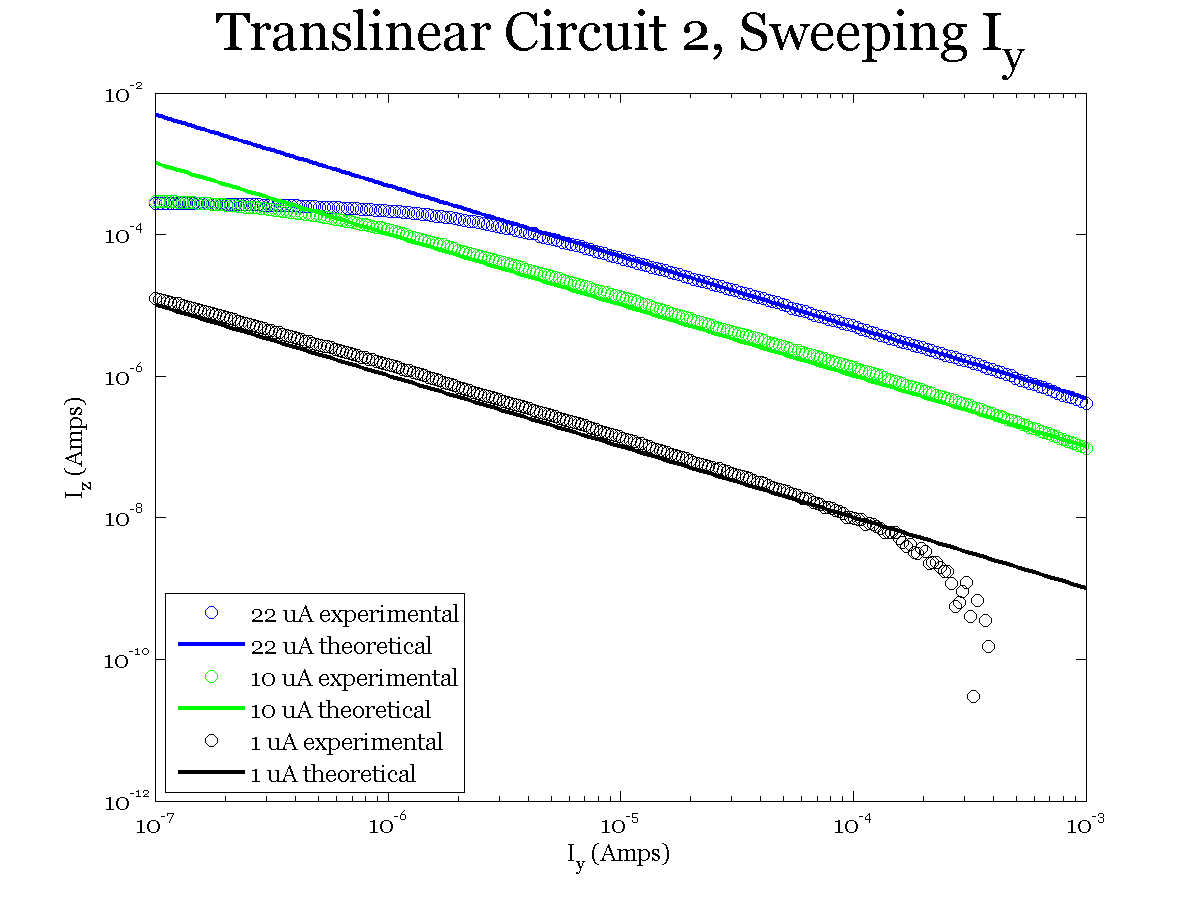
\includegraphics[scale=.75]{exp3_sweepy.png}
\caption{Translinear circuit 2, holding $I_x$ at the values shown in the legend.}
\label{fig:tl2sweepy}
\end{center}
\end{figure}

This was our worst-behaved configuration.  We found that we if we decreased $I_x$ below around 20 uA, $I_z$ was dominated by the non-linear region we believe is in error.  If we increased $I_x$ to more than 100 uA, we found that $I_z$ was very noisy for large input values.  As a result, we only measured $I_y$ for $I_x$ at values of 22 uA, 10 uA, and 100 uA.

\end{document}